\section{Beyond the $1+1$ qubit experiment}\label{sec:beyondMoreva}

In this Section, a closer look is given at the experimental illustration from \cite{Moreva:illustration};
and some original results are achieved in addition to the findings therein.
%
First, an explicit expression of the time operator $\op{T}$
is obtained.
The \mbox{paper} \parencite{Moreva:illustration}
only defines the frequency operator $\op{\Omega}$,
without exploring the relation between the two canonically conjugate operators
---which, in a finite-dimensional system, has some peculiarities, as seen in Sec.~\ref{sec:finite-quantum}.
%
A time eigenbasis is then identified, thus diagonalizing the related matrix.
%
Finally, a discrete-time evolution of the system of interest is computed from the Page--Wooters model,
and compared to the predictions of
standard quantum mechanics in continuous time.

\subsection{Time operator, diagonalization, evolution}
\label{1qubitExp}

The experiment described in \citereset\cite{Moreva:illustration}
reproduces the basic features of the Page--Wootters model
by identifying the overall state of the ``universe'' with an entangled state of the vertical
and
horizontal polarization degree of freedom of two photons
---as expressed in Eq.~\eqref{eq:moreva:overall_state}.
A {first} photon is identified as the ``clock'',
and the {second} one as the ``rest of the universe'',
in Page--Wootters sense.
The notation $\ket{H}_T, \ket{V}_T; \ket{H}_S, \ket{V}_S$
is used to refer to the horizontal and vertical polarization states of the two photons respectively.

Consistently to the Model, the experiment is prepared in such a way
as to show that the overall system $\dket{\Psi}$ ---Eq.~\eqref{eq:moreva:overall_state}---
is stationary,
i.e. it is in an eigenstate of the overall Hamiltonian $\op{\mathbb{J}}$ ---Eq.~\eqref{eq:pwHamiltonian}---;
while, ``internally'', the first photon can be interpreted as a clock for the ``evolution'' of the second one.

The authors choose, for their experiment,
a particular
frequency operator $\op{\Omega}$
defined by Eq.~\eqref{eq:MorevaOmegaT}.
Let us recall that it is $\hbar\op{\Omega} = \op{H}_T$,
i.e., up to a constant $\hbar$, the frequency operator is the ``Hamiltonian of the clock''.
With respect to the polarization basis of the first photon
$\qty{\ket{H}_T, \ket{V}_T}$,
the operator $\op{H}_T$ is then represented in matrix form as
\begin{equation}\label{eq:H_T}
  \op{H}_T = \hbar\op{\Omega} \repr {
    i\hbar\omega
    \begin{pmatrix}
      0 & 1 \\
     -1 & 0
    \end{pmatrix}
  } \, \text{.}
\end{equation}

As per the second photon (the ``rest of the universe''),
its Hamiltonian is defined as
\begin{equation}\label{eq:H_S}
  \op{H}_S \repr {
    i\hbar\omega
    \begin{pmatrix}
      0 & 1 \\
     -1 & 0
    \end{pmatrix}
  } \, \text{,}
\end{equation}
with respect to the polarization basis $\qty{\ket{H}_S, \ket{V}_S}$.

Note that there is no particular physical reason
(other than simplicity of realization)
for the matrices in Eq.~\eqref{eq:H_T} and \eqref{eq:H_S} to be formally identical.
They represent operators acting on two different Hilbert spaces, $\hilb{H}_T$ and $\hilb{H}_S$.
In another experiment,
in principle,
the clock may be described by a different definition of $\op{\Omega}$,
and there would be a
different expression for the overall stationary state;
$\hilb{H}_T$ and $\hilb{H}_S$ may even have different dimensions
---and so would the matrices representing $\op{H}_S$ and $\op{H}_T$ therein.

Back to the definitions of \citereset\cite{Moreva:illustration},
one can easily obtain
the spectrum of $\op{\Omega}$
as being comprised of eigenvalues
$\qty{-\omega, \omega}$.
Therefore, it is $N=2$ and $\delta\Omega = 2\omega$ in the sense of
\eqref{eq:SI_Fourier:T}.
We can thus derive the time operator matrix:
\begin{equation}
  \op{T}
  \repr
  \frac{\pi}{4\omega^2} F^{\dagger} \Omega F
  =
  \frac{i\pi}{8\omega}
  \begin{pmatrix}
    1 & 1 \\
    1 & -1
  \end{pmatrix}
  \begin{pmatrix}
    0 & 1 \\
   -1 & 0
  \end{pmatrix}
  \begin{pmatrix}
    1 & 1 \\
    1 & -1
  \end{pmatrix}
  =
  \frac{\pi}{4\omega}
  \begin{pmatrix}
    0 & -i \\
    i &  0
  \end{pmatrix}
  \,\text{.}
\end{equation}
We notice that time is not diagonal in the polarization basis.
It can be diagonalized with:
\begin{equation}\label{eq:moreva_diag_T}
  \mathcal{E}_T^{\dagger} T \mathcal{E}_T
  =
\frac{\pi}{4\omega}
\begin{pmatrix}
  -1  & 0 \\
  0   & 1
\end{pmatrix}
\,\text{,}
\end{equation}
and $\mathcal{E}_T$ being the matrix of eigenvectors of $\op{T}$ as columns
\begin{equation}
  \mathcal{E}_T
  =
  \frac{1}{\sqrt{2}}
  \begin{pmatrix}
    i & -i \\
    1 & 1
  \end{pmatrix}
  \,\text{.}
\end{equation}
Thus the clock can measure (only) the two times: $-\frac{\pi}{4\omega}$ and $\frac{\pi}{4\omega}$
(or superpositions of them):
\begin{align}
  \ket{-\frac{\pi}{4\omega}} &= \frac{1}{\sqrt{2}} \qty(\ket{V}+i\ket{H}) \eqbydef \ket{L} \\
  \ket{ \frac{\pi}{4\omega}} &= \frac{1}{\sqrt{2}} \qty(\ket{V}-i\ket{H}) \eqbydef \ket{R} \, \text{.}
\end{align}
In terms of the physics of the experiment,
time eigenstates coincide with
the two circular polarization states of the clock photon.

It's worth observing that
only if $\op{T}$ is diagonal in a certain basis $\qty{t}$,
the components of a vector in $\hilb{H}_T \ox \hilb{H}_S$
over that basis
can be interpreted as a ``time evolution'':
\begin{equation}\label{eq:timepicks2}
  \dket{\Psi}
  \repr_{\qty{t} \ox \qty{H,V}}
  \qty{\psi_H(t_0), \psi_V(t_0), \psi_H(t_1), \psi_V(t_1)}
\end{equation}
or, in general:
\begin{equation}\label{eq:timepicksN}
  \dket{\Psi}
  \repr
  \qty{
    \psi_0(t_0),
    \dotsc,
    \psi_{N_{S} - 1}(t_0),
    \dots,
    \psi_0(t_{N_{T}-1}),
    \dotsc,
    \psi_{N_{S} - 1}(t_{N_{T}-1})
  } \,\text{,}
\end{equation}
where
$t_0, t_1, \dots, t_{N_{T}-1}$ are the eigenvalues of the time operator,
and
$N_{S}$ and $N_{T}-1$ the dimensions of $\hilb{H}_T$ and $\hilb{H}_S$ respectively.

The basis of interest is therefore
\begin{equation}
  \qty{\ket{-\frac{\pi}{4\omega}}, \ket{\frac{\pi}{4\omega}}}_T \ox \qty{\ket{H}, \ket{V}}_S
  \, \text{.}
\end{equation}

How does the matrix of $\op{\Omega}$ transform? In general, it's
\begin{equation}
  \Omega \rightarrow F \mathcal{E}_T^{\dagger} F^{\dagger} \Omega F \mathcal{E}_T F^{\dagger}
  \, \text{,}
\end{equation}
but we already know $F^{\dagger} \Omega F = T$,
and $\mathcal{E}_T^{\dagger} T \mathcal{E}_T$ is the diagonal matrix
(let's call it $T_d$) of the \eqref{eq:moreva_diag_T}.
In conclusion, with some algebra, it's simply
\begin{equation}
  \Omega_{T_d} \eqbydef F^{\dagger} T_d F = \left(\begin{matrix}0 & - \omega\\- \omega & 0\end{matrix}\right)
\end{equation}
and we are interested in the eigensystem of
\begin{multline}
  \mathbb{J}_{T_d} \eqbydef \hbar \Omega_{T_d} \ox \idop_{S} + \idop_{T_d} \ox H_S =
    \hbar
    \begin{pmatrix}0 & - \omega\\- \omega & 0\end{pmatrix}
    \ox
    \begin{pmatrix} 1 & 0 \\  0 & 1 \end{pmatrix}
    + \\
    \hbar\omega
    \begin{pmatrix} 1 & 0 \\  0 & 1 \end{pmatrix}
    \ox
    \begin{pmatrix} 0 & 1 \\ -1 & 0 \end{pmatrix}
    =
    \hbar\omega
    \begin{pmatrix}
      0   &i  &-1 &0  \\
      -i  &0  &0  &-1 \\
      -1  &0  &0  &i  \\
      0   &-1 &-i &0  
    \end{pmatrix}
  \text{,}
\end{multline}
which is
\begin{align}
  j_0     &= 0\,\text{;}              &\ket{j_{0}1}   \repr (0, -i, 1, 0) \quad \ket{j_0 2} \repr (i, 0, 0 ,1)
    \label{eq:moreva:eigenJ0} \\
  j_{-1}  &= -2\hbar\omega\,\text{;}  &\ket{j_{-1}}   \repr (-i, 1, -i, 1) \\
  j_{+1}   &= 2\hbar\omega\,\text{;}  &\ket{j_{+1}}   \repr (-i, -1, i, 1)
\end{align}

See \ref{nb:jupyter:moreva} for more details.


\subsection{Consistency with predictions of ordinary quantum theory}
\label{sec:qubit:pw-vs-qm}

In ordinary quantum theory, time is an absolute, external, ``classical'' \emph{parameter},
with respect to $\ket{\psi} \in \hilb{H}_S$; and $\hilb{H}_S$
is the only Hilbert space under consideration.

For each value of $t \in \mathbb{R}$ there is
\begin{equation}\label{eq:ordinary_evolution}
  \ket{\psi(t)}_{\text{Schr\"od.}} =
  %\sum_{k=H,V}\ket{k}\braket{k}{\psi(t)} =
  e^{-i\op{H}_{S}(t-t_0)/\hbar}\ket{\psi(t_0)}
\end{equation}

In terms of the Page and Wootters model,
let's pick instead as an example the first eigenstate in \eqref{eq:moreva:eigenJ0}.
It's related to a time operator whose eigenvalues are
$-\frac{\pi}{4\omega}, \frac{\pi}{4\omega}$
per Eq.~\eqref{eq:moreva_diag_T}.
The vector $(0, -i, 1, 0)$ indicates ---in ordinary quantum mechanics terms---
the following time evolution:
\begin{equation}
  \ket{\psi\qty(-\frac{\pi}{4\omega})} = -i\ket{V}
  \quad \rightarrow \quad
  \ket{\psi\qty( \frac{\pi}{4\omega})}_{\mathrm{PW}} =   \ket{H}
  \, \text{,}
\end{equation}
while the standard time evolution \eqref{eq:ordinary_evolution}, if we put
$t_0 = -\frac{\pi}{4\omega}$, $t = \frac{\pi}{4\omega}$, $\ket{\psi\qty(t_0)} = -i\ket{V}$,
yields (see \ref{nb:jupyter:moreva:qm}):
\begin{equation}
  \ket{\psi\qty(-\frac{\pi}{4\omega})} = -i\ket{V}
  \quad \rightarrow \quad
  \ket{\psi\qty( \frac{\pi}{4\omega})}_{\mathrm{Schr\ddot{o}d.}} = -i\ket{H}
  \, \text{,}
\end{equation}
showing that the two theories are consistent \emph{up to a phase} factor
$e^{-i\omega'(t - t_{0})}$
\begin{equation}
  \ket{\psi(t)}_{\mathrm{PW}} e^{-i\omega'(t - t_{0})} = \ket{\psi(t)}_{\mathrm{Schr\ddot{o}d.}} \,\text{,}  
\end{equation}
with $\omega' = -\omega$ in this case.

A pattern that emerges in the general case is
\[
  \omega' \eqbydef \omega_{T_{0}} = \frac{\pi T_0}{(\delta T)^2} \,\text{,}
\]
where it is emphasized that this frequency shift is related to the clock starting
with a ground eigenvalue $T_0 \ne 0$.

A further generalization would consider non-zero eigenvalues $j$ of $\op{\mathbb{J}}$
(or $\epsilon$ in \cite[eq. 16]{Lloyd:Time}):
\begin{equation}\label{eq:pw-vs-qm}
  \ket{\psi(t)}_{\mathrm{PW}} e^{-i\omega_{j}(t - t_{0})} e^{-i\omega_{T_0}(t - t_{0})} = \ket{\psi(t)}_{\mathrm{Schr\ddot{o}d.}} \,\text{,}
\end{equation}
where $\hbar\omega_j = \epsilon$,
and $\mathbb{J}\dket{\Psi} = \epsilon \dket{\Psi}$
for the corresponding vector in $\hilb{H}_T \ox \hilb{H}_S$.

Physically, both correction terms merely
correspond to ``rigidly shifting the spectrum of $H_S$'' \parencite{Lloyd:Time}.
Predictions about a general probability distribution
$\abs{\braket{\xi}{\psi(t)}}^2$
are identical in the two models with no need of any phase/frequency correction term.\footnote{
  Where it's $\xi \in \qty{H, V}$
  in our case to represent linerar polarization states of the photon in
  the ``spatial'' Hilbert space $\hilb{H}_S$
  for the experiment.
}

\begin{spacing}{1.5}
  In \ref{nb:moreva-vs-qm},
  both sides of \eqref{eq:pw-vs-qm} are
  explicitely computed numerically and compared graphically.
  The left side (Page and Wootters)
  for $t = -\frac{\pi}{4\omega}, \frac{\pi}{4\omega}$ and also with
  $t = \frac{3\pi}{4\omega}$, identified with $t = -\frac{\pi}{4\omega}$
  to ``complete the cycle''.
  The right side (Schr{\"o}dinger) for
  $t \in \left[-\frac{\pi}{4\omega}, \frac{3\pi}{4\omega}\right[$.
\end{spacing}

Fig. \ref{fig:psi_H} and \ref{fig:psi_V} show
Page--Wootters discrete points, along with
ordinary Schr{\"o}dinger evolution (continuous curve)
of the photon polarization components
$\braket{H,V}{\psi(t)}$
from time $t = -\frac{\pi}{4\omega}$
to $t = \frac{3\pi}{4\omega}$. Time is on the $z$ axis,
while $x, y$ axis represent real and imaginary part of
the ``wavefunction'' values $\braket{H,V}{\psi(t)}$.
The straight line along the $z$ axis
spans the time period of interest
and is intersected when\footnote{
  ``When'' is a concept to be taken with a grain of salt in the Page--Wootters model.
  An hypothetical super-observer, outside of the Universe,
  who is real in our experiment ---being that just a toy universe---
  will only see a mixed state of all times on the clock photon, and the other
  photon being ``timed'' would represent its \emph{purification space}
  via entanglement.
}
the probability of the photon being
horizontally [vertically] polarized is zero.
Phase correction as per \eqref{eq:pw-vs-qm} has been taken into account
and we have scaled $\omega=1$.

\begin{figure}
  %\centering
  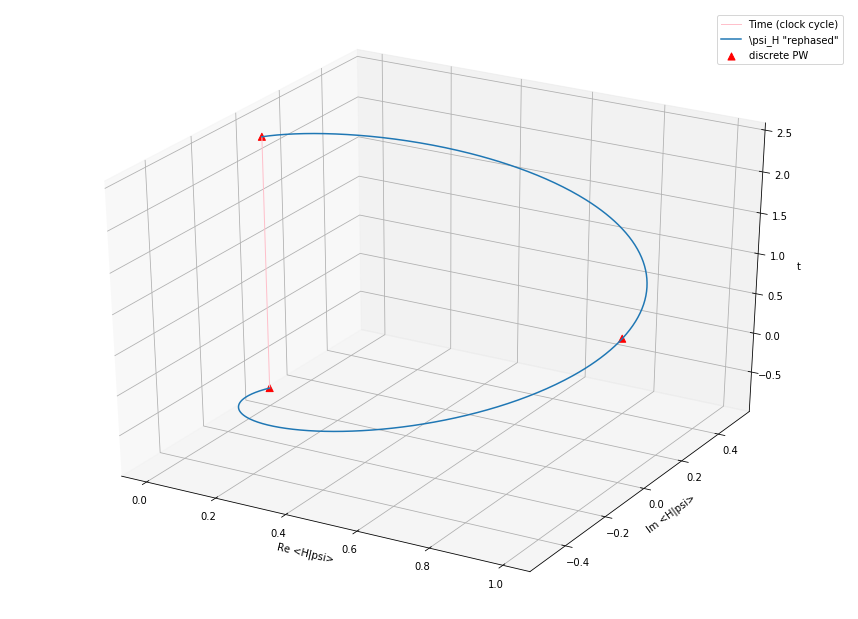
\includegraphics[width=\textwidth]{img/psi_H.png}
  \caption{
    Evolution of $\braket{H}{\psi(t)}$ in the two models.
  }
  \label{fig:psi_H}
\end{figure}

\begin{figure}
  %\centering
  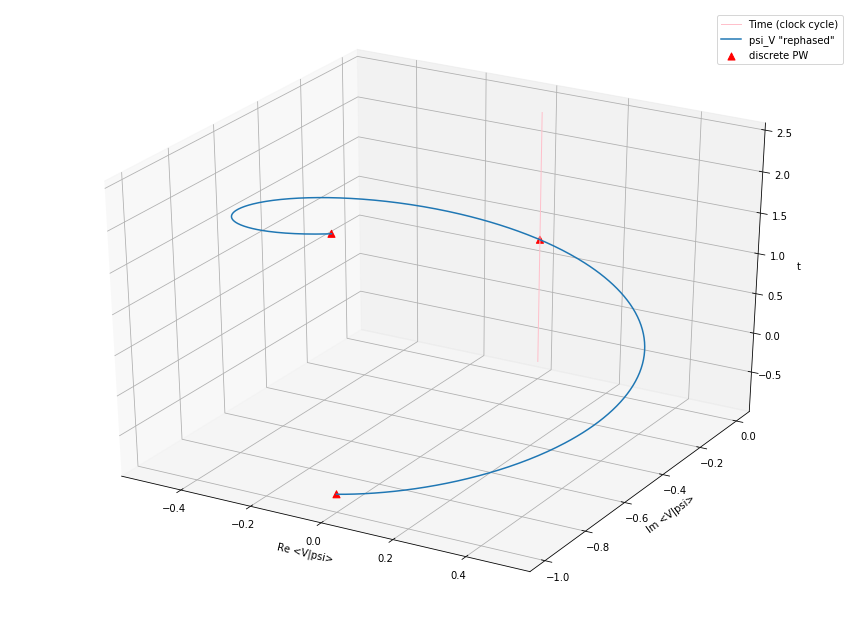
\includegraphics[width=\textwidth]{img/psi_V.png}
  \caption{Evolution of $\braket{V}{\psi(t)}$ in the two models.}
  \label{fig:psi_V}
\end{figure}
